\chapter{Discipline and Procrastination}

This chapter follows a Jim Rohn lecture preserved in a curated LazyingArt LLC playlist. There is no usable board evidence for this talk, so the mathematical structure has to be drawn from the speech itself. Fortunately the opening is unusually precise. We are asked to look first at a relation between awareness and action, then at the delay that breaks that relation, then at the very different lives that grow from the two cases. If we keep that thread in hand, the rest of the lecture unfolds with surprising coherence: reward timing, distraction, consistency, standards, multiplication of return, and finally the judgment that a life becomes either a warning or an example.

\section{Discipline and Procrastination as a Time Relation}

The lecture begins with a definition, and it repeats the definition almost verbatim. That repetition is not filler. It fixes the governing law. Discipline is not first treated as temperament, enthusiasm, or even moral heroism. It is treated as a joining of two moments: we become aware that action is needed, and then we consciously implement that action.

\begin{equation}
D := (\text{awareness of the need for action}) + (\text{conscious implementation of that action}).
\end{equation}

If we want a compact editorial notation for the lecturer's opening contrast, we may introduce a lag between awareness and implementation:
\begin{equation}
\Delta t := t_{\mathrm{impl}} - t_{\mathrm{aware}}.
\end{equation}
The notation is ours rather than his, but it captures the point cleanly. When awareness and implementation occur together, a valued sequence of disciplined activity begins. When a considerable time passes between them, the name of the process changes:
\begin{align}
\Delta t \approx 0 &\Rightarrow \text{disciplined activity}, \\
\Delta t \gg 0 &\Rightarrow \text{procrastination}.
\end{align}

With no validated lecture-board frame for this talk, the following figure is editorial. It simply makes visible the timing structure that the lecture states in words.

\begin{figure}
\centering
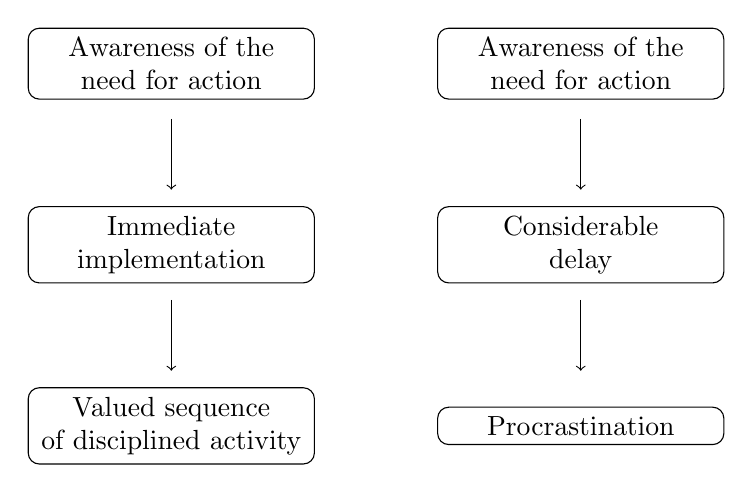
\begin{tikzpicture}[x=1cm,y=1cm]
\node[draw, rounded corners, align=center, text width=3.4cm] at (-2.6,0) {Awareness of the\\need for action};
\node[draw, rounded corners, align=center, text width=3.4cm] at (-2.6,-2.3) {Immediate\\implementation};
\node[draw, rounded corners, align=center, text width=3.4cm] at (-2.6,-4.6) {Valued sequence\\of disciplined activity};

\node[draw, rounded corners, align=center, text width=3.4cm] at (2.6,0) {Awareness of the\\need for action};
\node[draw, rounded corners, align=center, text width=3.4cm] at (2.6,-2.3) {Considerable\\delay};
\node[draw, rounded corners, align=center, text width=3.4cm] at (2.6,-4.6) {Procrastination};

\draw[->] (-2.6,-0.7) -- (-2.6,-1.6);
\draw[->] (-2.6,-3.0) -- (-2.6,-3.9);
\draw[->] (2.6,-0.7) -- (2.6,-1.6);
\draw[->] (2.6,-3.0) -- (2.6,-3.9);
\end{tikzpicture}
\end{figure}

The lecture immediately translates this structure into ordinary speech. The inward voice says, get it done. Discipline answers, do it now. Procrastination answers, later, tomorrow, whenever I get a chance. So the slogan is not a simplification away from the structure. It is the structure carried into daily language.

\subsection{Question \& Answer}

Question. What exactly separates discipline from procrastination?

Answer. Not knowledge alone, and not desire alone. In both cases we may know what must be done. The difference is whether action joins awareness or separates from it. Discipline closes the interval. Procrastination widens it.

\paragraph{Worked comparison.}
We can write the lecture's opening logic as a short progression.
\begin{enumerate}
\item Awareness of a needed action occurs.
\item Implementation either follows promptly or does not.
\item If implementation joins awareness, disciplined activity begins.
\item If implementation is deferred by a substantial lag, the same situation is renamed procrastination.
\end{enumerate}

\section{Do It Now or Do It Later: Fruit and Reward Timing}

Once the opening relation has been fixed, the lecture widens it into a contrast between kinds of life. Discipline is no longer only promptness; it is a disciplined existence, one that bears the fruit of achievement and contentment. Procrastination is not only delay; it becomes the easy life, a life that bears no fruit, only the bare branches of mediocrity. The line immediately before this image is corrupted, but the image itself is clear and should be preserved:
\begin{equation}
\text{discipline} \Rightarrow \text{achievement and contentment}, \qquad
\text{procrastination} \Rightarrow \text{bare branches of mediocrity}.
\end{equation}

The whole contrast is then compressed into the lecture's most portable pair:
\begin{equation}
\text{discipline} \leftrightarrow \text{do it now}, \qquad
\text{procrastination} \leftrightarrow \text{do it later}.
\end{equation}
The speaker then makes a subtle move. He lets procrastination speak not only as delay but as a philosophy of minimum obligation: do what is necessary to get by, do what you can, but not what you must. That gives the later reward analysis its proper target. We are not comparing effort with idleness in the abstract. We are comparing two rival schedules of reward and two rival standards of conduct.

\begin{equation}
\text{rewards of discipline} = \text{great but delayed}, \qquad
\text{rewards of lack of discipline} = \text{immediate but minor}.
\end{equation}
The beach comparison is the lecture's way of making this vivid:
\begin{equation}
\text{immediate reward of indiscipline} = \text{a fun day at the beach}, \qquad
\text{future reward of discipline} = \text{owning the beach}.
\end{equation}
This is not economics. It is moral arithmetic. The smaller reward arrives sooner. The larger reward arrives later. The wrong path remains tempting precisely because it pays quickly.

A compact shorthand for the lecturer's description of common choice is
\begin{equation}
\text{today's pleasure} > \text{tomorrow's fortune},
\end{equation}
not as a rule we should admire, but as an account of what most of us too often prefer.

\subsection{Question \& Answer}

Question. If indiscipline feels rewarding now, why is it not the better bargain?

Answer. Because the lecture's comparison is between two reward schedules, not between reward and emptiness. The easy path pays at once, but it pays little. The disciplined path delays payment, but the return is larger by order of magnitude. So the nearness of the reward is the trap.

\section{Distraction, Focus, and the Power of Association}

At this point the lecture stops stating principles and begins pressing questions. How do we get rid of easy distractions? How do we keep the mind on what we are trying to do? How do we maintain the attitude of doing it all, and doing it now? How do we choose discipline over procrastination? How do we avoid the water cooler? The rapid questioning matters. The lecture wants us to feel the pressure of application, not merely to admire the distinction already made.

The initial answer is direct: keep the focus on the work, get it done today instead of tomorrow, and work on consistent self-discipline daily. But the lecturer quickly shows that distraction is not one thing. It comes as a cluster:
\begin{equation}
(\text{negative thoughts},\ \text{negative people},\ \text{water-cooler chatter},\ \text{doubts within oneself}).
\end{equation}
That list is important because it prevents us from imagining that discipline is only an inward act of will. We are also dealing with environments, associations, talk, mood, and the slow contamination of attention.

The lecture is especially sharp about the power of influence and association. Depending on the sort of people around us, we will be distracted. But the speaker puts the answer on the other side as well: never underestimate the power of our own consistent self-discipline. The contest is therefore asymmetrical but not hopeless. Social and mental noise widen the interval between awareness and implementation; daily discipline closes it again.

\subsection{Question \& Answer}

Question. How do distractions and associations actually defeat disciplined action?

Answer. They do not usually erase knowledge. They interfere with execution. The needed act remains visible, but it is deferred by chatter, social drag, inward doubt, and the lure of easier motions. So once again the issue is the size of the interval between awareness and implementation.

\section{The Three Steps and the First One: Discipline Is Not the Easiest Option}

Now the lecture announces that it will take a closer look at discipline through three steps. The three are not developed in perfectly clean order, but the structure is real. In editorial shorthand we may record it as
\begin{equation}
S_3 := (\text{discipline is not the easiest option},\ \text{discipline is a full-time activity},\ \text{every disciplined effort brings a multiple reward}).
\end{equation}
The first step is then developed at once:
\begin{equation}
\text{true discipline} \neq \text{the easiest option}.
\end{equation}

The lecture unpacks that claim by listing what is easier: sleeping until ten rather than rising at six, going to bed late, showing up late, leaving early, turning on the television rather than opening a book, doing just enough rather than doing it all. Two aphorisms condense the pattern:
\begin{equation}
\text{waiting is easier than acting}, \qquad \text{trying is easier than doing}.
\end{equation}
The examples are ordinary on purpose. The lecturer wants us to see that difficulty is not an exception attached to discipline from outside. It belongs to discipline from the start.

That is why the rhetorical question arrives exactly here. What would become of us if we did not have to make the bed, keep the garage clean, pay taxes, or show up for work? The answer is immediate: not much. And from there the lecture makes its broader claim:
\begin{equation}
\text{the easiest things in life} \Rightarrow \text{the most unprofitable}, \qquad
\text{the profitable} \Rightarrow \text{the most difficult}.
\end{equation}
The word ``profitable'' must not be over-read. This is not formal economics. It is the lecturer's way of saying that the world is arranged so that ease carries momentary rewards, while discipline carries the larger and more significant ones.

The point is then restated as a world-picture:
\begin{equation}
\text{life} = \text{battle between ease with momentary rewards and discipline with significant rewards}.
\end{equation}
And that battle has a price structure. The lecture's own verbal formula should be preserved: there is the price of discipline or the price of regret. We will pay one or the other. If one wants a compact editorial inequality, one may write
\begin{equation}
\text{price of discipline} < \text{price of regret},
\end{equation}
but the speaker's own closure is sharper in words: discipline costs pennies, regret costs a fortune.

\subsection{Question \& Answer}

Question. Why is the easiest option usually the least profitable one?

Answer. Because the easy act spares the immediate effort but not the eventual cost. The lecture's point is that ease pays quickly and then closes down the future, while discipline costs now and opens the future. Regret is therefore not an extra punishment added afterward; it is the long bill for preferring ease in each local decision.

\section{Second Step: Full-Time Consistency, Standards, and Credibility}

The transcript becomes unstable for a short stretch after the price-of-regret section, but when the lecture returns to clear ground it does so by naming the best form of discipline:
\begin{equation}
\text{best form of discipline} = \text{consistent self-discipline}.
\end{equation}
The examples once again are homely. The discipline required to make the bed each day is the same discipline required for success in business. The discipline needed to organize the garage is the same discipline required to organize the business. The point is not that the tasks are equal; it is that the structure of discipline carries through.

\begin{align}
\text{discipline in one area} &\Rightarrow \text{discipline in larger areas}, \\
\text{lazy side} &\to \text{destroys disciplined side}.
\end{align}
The second line is the more unsettling one. The lecture does not merely claim that order spreads. It claims that disorder spreads as well. If we are disciplined in one region and lazy in another, then the lazy side will creep in and destroy the disciplined side. Hence the maxim
\begin{equation}
\text{consistency cannot be inconsistent}.
\end{equation}
The phrase sounds circular, but the meaning is firm: consistency is not a local decoration on one or two tasks. It is a property of the whole pattern of conduct.

This allows the lecture to deepen its earlier definition:
\begin{equation}
\text{discipline} := \text{the mind being trained to control our lives}.
\end{equation}
And immediately after that, the speaker turns from habit to law. We select standards as a personal code of conduct:
\begin{equation}
C := \text{a selected personal code of conduct}.
\end{equation}
Then discipline acquires a second, more juridical formulation:
\begin{equation}
\text{discipline} := \text{imposing on ourselves the requirements for honoring our standards}.
\end{equation}
That shift is important. Discipline is now no longer mere repetition. It is fidelity to a chosen code.

The natural next target is hypocrisy. We announce beliefs, instruct children, instruct employees, and yet do not walk the talk. The lecture treats this not merely as embarrassment, but as structural failure:
\begin{equation}
\text{announced standards} \land \text{unlived conduct} \Rightarrow \text{loss of credibility outwardly and inwardly}.
\end{equation}
The outer loss is obvious enough. Others stop trusting our words. The deeper loss is inward. We cease to trust ourselves as people who honor the code we claim to live by.

The lecture sharpens the point further by giving a darker portrait. Worse than the inconsistent disciplinarian is the person who has never considered the need or value of discipline at all. Such a life wanders from commitment to commitment and leaves behind the usual wreckage:
\begin{equation}
\text{no sense of the need or value of discipline} \Rightarrow \text{wandering commitments} + \text{broken friendships} + \text{unfinished projects} + \text{unfulfilled promises}.
\end{equation}
So the lecture has now moved from time relation, to reward, to global consistency, and finally to the moral texture of a life.

\subsection{Question \& Answer}

Question. What breaks first when our standards are declared but not lived?

Answer. Credibility breaks first, and it breaks in two directions. Others lose trust in our words, and we lose trust in our own capacity to honor the standards we have chosen. That is why the lecturer treats inconsistency as more than inefficiency. It is a fracture in self-government.

\subsection{Question \& Answer}

Question. Can discipline remain local to one area while we are lazy in another?

Answer. The lecture's answer is no. The same pattern that orders one part of life migrates into the others, and the same is true of disorder. That is why consistent self-discipline is not occasional heroism but a full-time condition.

\paragraph{Transfer rule.}
The lecture's spillover logic can be written in five short steps.
\begin{enumerate}
\item A discipline is established in a small daily area.
\item That discipline shapes the way we meet ordinary obligations.
\item The same structure appears in larger responsibilities.
\item A protected lazy region spreads by the same mechanism.
\item Therefore discipline must be treated as global rather than compartmental.
\end{enumerate}

\section{Third Step: Multiple Reward, Boundaries, and Self-Imposed Discipline}

Only after the cost of ease and the demand for consistency have been worked through does the lecture name the third step. That sequencing matters. The promise is allowed to arrive only after the seriousness of the problem has been felt.

The third step is the lecture's second major law:
\begin{equation}
\text{for every disciplined effort, there is a multiple reward}.
\end{equation}
The line is repeated several times in the talk, and it should remain repeated in spirit in the notes. The speaker wants it to sink in as one of life's great arrangements. He ties it at once to sowing and reaping:
\begin{equation}
\text{if you sow well, you reap well}, \qquad
\text{we reap what we've sown and we reap much more}.
\end{equation}
The key addition is the second clause. It is not only that action returns its own measure. It returns multiplied.

This is then unfolded through examples. If we render unique service, the reward is multiplied. If we are fair, honest, and patient with others, the reward is multiplied. If we give more than we expect to receive, the reward is more than we expect. The repeated formula is not an ornamental slogan but the lecture's law of moral increase.

The talk then widens this law beyond business and reward language. Everything of value requires care and attention; everything of value requires discipline.
\begin{equation}
\text{everything of value requires care and attention}, \qquad
\text{everything of value requires discipline}.
\end{equation}
Children require discipline. Thoughts require discipline.
\begin{equation}
\text{children require discipline}, \qquad \text{thoughts require discipline}.
\end{equation}
The parallel matters. Children need boundaries in order to grow securely. Thoughts need boundaries in order not to become confused. And from this the lecturer draws a crisp cognitive consequence:
\begin{equation}
\text{confused thoughts} \Rightarrow \text{confused results}.
\end{equation}
Discipline is therefore not merely constraint. It is form. It creates the bounded field within which growth and clear action are possible.

The lecture then turns personal once more. The most valuable form of discipline is the discipline one imposes on oneself:
\begin{equation}
\text{most valuable discipline} = \text{the discipline one imposes on oneself}.
\end{equation}
That line closes the circle. The opening definition described discipline operationally, as awareness joined to implementation. The ending describes it morally and politically, as self-government. To wait until someone else imposes discipline is, in the lecturer's language, tragic, because it means another person thought more of our order than we did.

The final classification of lives then follows naturally:
\begin{equation}
\text{life} \in \{\text{warning},\ \text{example}\}.
\end{equation}
A life may warn by neglect, self-pity, lack of direction, and abandoned promise. Or it may exemplify talent put to use, discipline self-imposed, and aims intensely pursued. The transcript frays at the very end, but this final contrast is clear and should stand.

\subsection{Question \& Answer}

Question. Why does self-imposed discipline yield more than it seems to cost?

Answer. Because in the lecture self-imposed discipline is not a subtractive act. It is seed-like. It yields steadier action, stronger credibility, clearer thought, better boundaries, and multiplied return. External discipline may still create order, but it arrives late and at a moral loss.

\paragraph{Boundary principle.}
The lecture applies one structure in two domains.
\begin{enumerate}
\item Children need boundaries so that growth can take place within order rather than confusion.
\item Thoughts need boundaries so that judgment can occur within shape rather than drift.
\item In both cases discipline is not the enemy of life but its scaffolding.
\end{enumerate}

\section{Summary}

The lecture begins with a precise relation and ends with a judgment on lives. First, discipline is awareness joined to implementation, while procrastination is the lag between the two. Then the speaker widens the contrast into a difference between lives: fruit or bare branches, delayed large rewards or immediate small ones, discipline or regret. From there he moves through distraction, association, the refusal of ease, the demand for consistency, the honoring of standards, the danger of hypocrisy, and finally the law that disciplined effort multiplies its return.

What holds the chapter together is that every later claim can be traced back to the opening relation. If awareness and action are separated, mediocrity begins to accumulate. If they are joined, disciplined activity begins to accumulate. The lecture never really leaves that first distinction; it simply keeps unfolding its consequences until it can say, at the end, that our lives will stand either as warnings or as examples.